\documentclass[twoside]{book}

% Packages required by doxygen
\usepackage{fixltx2e}
\usepackage{calc}
\usepackage{doxygen}
\usepackage[export]{adjustbox} % also loads graphicx
\usepackage{graphicx}
\usepackage[utf8]{inputenc}
\usepackage{makeidx}
\usepackage{multicol}
\usepackage{multirow}
\PassOptionsToPackage{warn}{textcomp}
\usepackage{textcomp}
\usepackage[nointegrals]{wasysym}
\usepackage[table]{xcolor}

% Font selection
\usepackage[T1]{fontenc}
\usepackage[scaled=.90]{helvet}
\usepackage{courier}
\usepackage{amssymb}
\usepackage{sectsty}
\renewcommand{\familydefault}{\sfdefault}
\allsectionsfont{%
  \fontseries{bc}\selectfont%
  \color{darkgray}%
}
\renewcommand{\DoxyLabelFont}{%
  \fontseries{bc}\selectfont%
  \color{darkgray}%
}
\newcommand{\+}{\discretionary{\mbox{\scriptsize$\hookleftarrow$}}{}{}}

% Page & text layout
\usepackage{geometry}
\geometry{%
  a4paper,%
  top=2.5cm,%
  bottom=2.5cm,%
  left=2.5cm,%
  right=2.5cm%
}
\tolerance=750
\hfuzz=15pt
\hbadness=750
\setlength{\emergencystretch}{15pt}
\setlength{\parindent}{0cm}
\setlength{\parskip}{3ex plus 2ex minus 2ex}
\makeatletter
\renewcommand{\paragraph}{%
  \@startsection{paragraph}{4}{0ex}{-1.0ex}{1.0ex}{%
    \normalfont\normalsize\bfseries\SS@parafont%
  }%
}
\renewcommand{\subparagraph}{%
  \@startsection{subparagraph}{5}{0ex}{-1.0ex}{1.0ex}{%
    \normalfont\normalsize\bfseries\SS@subparafont%
  }%
}
\makeatother

% Headers & footers
\usepackage{fancyhdr}
\pagestyle{fancyplain}
\fancyhead[LE]{\fancyplain{}{\bfseries\thepage}}
\fancyhead[CE]{\fancyplain{}{}}
\fancyhead[RE]{\fancyplain{}{\bfseries\leftmark}}
\fancyhead[LO]{\fancyplain{}{\bfseries\rightmark}}
\fancyhead[CO]{\fancyplain{}{}}
\fancyhead[RO]{\fancyplain{}{\bfseries\thepage}}
\fancyfoot[LE]{\fancyplain{}{}}
\fancyfoot[CE]{\fancyplain{}{}}
\fancyfoot[RE]{\fancyplain{}{\bfseries\scriptsize Generated by Doxygen }}
\fancyfoot[LO]{\fancyplain{}{\bfseries\scriptsize Generated by Doxygen }}
\fancyfoot[CO]{\fancyplain{}{}}
\fancyfoot[RO]{\fancyplain{}{}}
\renewcommand{\footrulewidth}{0.4pt}
\renewcommand{\chaptermark}[1]{%
  \markboth{#1}{}%
}
\renewcommand{\sectionmark}[1]{%
  \markright{\thesection\ #1}%
}

% Indices & bibliography
\usepackage{natbib}
\usepackage[titles]{tocloft}
\setcounter{tocdepth}{3}
\setcounter{secnumdepth}{5}
\makeindex

% Hyperlinks (required, but should be loaded last)
\usepackage{ifpdf}
\ifpdf
  \usepackage[pdftex,pagebackref=true]{hyperref}
\else
  \usepackage[ps2pdf,pagebackref=true]{hyperref}
\fi
\hypersetup{%
  colorlinks=true,%
  linkcolor=blue,%
  citecolor=blue,%
  unicode%
}

% Custom commands
\newcommand{\clearemptydoublepage}{%
  \newpage{\pagestyle{empty}\cleardoublepage}%
}

\usepackage{caption}
\captionsetup{labelsep=space,justification=centering,font={bf},singlelinecheck=off,skip=4pt,position=top}

%===== C O N T E N T S =====

\begin{document}

% Titlepage & ToC
\hypersetup{pageanchor=false,
             bookmarksnumbered=true,
             pdfencoding=unicode
            }
\pagenumbering{roman}
\begin{titlepage}
\vspace*{7cm}
\begin{center}%
{\Large My Project }\\
\vspace*{1cm}
{\large Generated by Doxygen 1.8.11}\\
\end{center}
\end{titlepage}
\clearemptydoublepage
\tableofcontents
\clearemptydoublepage
\pagenumbering{arabic}
\hypersetup{pageanchor=true}

%--- Begin generated contents ---
\chapter{File Index}
\section{File List}
Here is a list of all files with brief descriptions\+:\begin{DoxyCompactList}
\item\contentsline{section}{\hyperlink{Lab1_8c}{Lab1.\+c} }{\pageref{Lab1_8c}}{}
\end{DoxyCompactList}

\chapter{File Documentation}
\hypertarget{ArrayPractice_8cpp}{}\section{Array\+Practice.\+cpp File Reference}
\label{ArrayPractice_8cpp}\index{Array\+Practice.\+cpp@{Array\+Practice.\+cpp}}
{\ttfamily \#include $<$iostream$>$}\\*
Include dependency graph for Array\+Practice.\+cpp\+:
\nopagebreak
\begin{figure}[H]
\begin{center}
\leavevmode
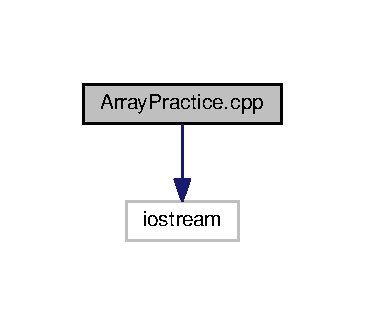
\includegraphics[width=175pt]{ArrayPractice_8cpp__incl}
\end{center}
\end{figure}
\subsection*{Functions}
\begin{DoxyCompactItemize}
\item 
void \hyperlink{ArrayPractice_8cpp_ad637601aeb87032b931bc689000f503a}{reverse} (const char a\mbox{[}$\,$\mbox{]}, int num\+\_\+used)
\item 
int \hyperlink{ArrayPractice_8cpp_ab8338266524a19fa4f8d74cd8bc6b6a6}{compute\+\_\+average} (const int a\mbox{[}$\,$\mbox{]}, int num\+\_\+used)
\item 
void \hyperlink{ArrayPractice_8cpp_aa3a5d4ca3a58aa1b5c5c94668cbdd8fd}{fill\+\_\+array} (char a\mbox{[}$\,$\mbox{]}, int size, int \&num\+\_\+used)
\item 
void \hyperlink{ArrayPractice_8cpp_a6f6feac3e7a1b1b1f121e0202e1b51e3}{fill\+\_\+array} (int a\mbox{[}$\,$\mbox{]}, int size)
\item 
int \hyperlink{ArrayPractice_8cpp_ad5f309c4942b742af6f5a4d95b15ae00}{find\+\_\+max} (int a\mbox{[}$\,$\mbox{]}, int num\+\_\+used, int \&max\+\_\+index)
\item 
void \hyperlink{ArrayPractice_8cpp_a7f37f8fb77dfd2e0d06f665c7dad4d6f}{find\+\_\+max\+\_\+min} (int a\mbox{[}$\,$\mbox{]}, int num\+\_\+used, int \&max\+\_\+index, int \&min\+\_\+index)
\item 
int \hyperlink{ArrayPractice_8cpp_ae66f6b31b5ad750f1fe042a706a4e3d4}{main} ()
\end{DoxyCompactItemize}


\subsection{Function Documentation}
\index{Array\+Practice.\+cpp@{Array\+Practice.\+cpp}!compute\+\_\+average@{compute\+\_\+average}}
\index{compute\+\_\+average@{compute\+\_\+average}!Array\+Practice.\+cpp@{Array\+Practice.\+cpp}}
\subsubsection[{\texorpdfstring{compute\+\_\+average(const int a[], int num\+\_\+used)}{compute_average(const int a[], int num_used)}}]{\setlength{\rightskip}{0pt plus 5cm}int compute\+\_\+average (
\begin{DoxyParamCaption}
\item[{const int}]{a\mbox{[}$\,$\mbox{]}, }
\item[{int}]{num\+\_\+used}
\end{DoxyParamCaption}
)}\hypertarget{ArrayPractice_8cpp_ab8338266524a19fa4f8d74cd8bc6b6a6}{}\label{ArrayPractice_8cpp_ab8338266524a19fa4f8d74cd8bc6b6a6}

\begin{DoxyCode}
65 \{
66    \textcolor{keywordtype}{int} sum = 0;
67    \textcolor{keywordflow}{for} (\textcolor{keywordtype}{int} k = 0; k < num\_used; k++)
68    \{
69       sum += a[k];
70    \}
71    \textcolor{keywordflow}{return} sum/num\_used;
72 \}
\end{DoxyCode}
\index{Array\+Practice.\+cpp@{Array\+Practice.\+cpp}!fill\+\_\+array@{fill\+\_\+array}}
\index{fill\+\_\+array@{fill\+\_\+array}!Array\+Practice.\+cpp@{Array\+Practice.\+cpp}}
\subsubsection[{\texorpdfstring{fill\+\_\+array(char a[], int size, int \&num\+\_\+used)}{fill_array(char a[], int size, int &num_used)}}]{\setlength{\rightskip}{0pt plus 5cm}void fill\+\_\+array (
\begin{DoxyParamCaption}
\item[{char}]{a\mbox{[}$\,$\mbox{]}, }
\item[{int}]{size, }
\item[{int \&}]{num\+\_\+used}
\end{DoxyParamCaption}
)}\hypertarget{ArrayPractice_8cpp_aa3a5d4ca3a58aa1b5c5c94668cbdd8fd}{}\label{ArrayPractice_8cpp_aa3a5d4ca3a58aa1b5c5c94668cbdd8fd}

\begin{DoxyCode}
32 \{
33    \textcolor{keywordtype}{char} c;
34    num\_used = 0;
35    cout << \textcolor{stringliteral}{"Enter up to 10 characters. Enter ';' to stop: "};
36    \textcolor{keywordflow}{for} (\textcolor{keywordtype}{int} k = 0; k < size; k++)
37    \{
38       cin >> c;
39       \textcolor{keywordflow}{if} (c == \textcolor{charliteral}{';'})
40          \textcolor{keywordflow}{break};
41       a[k] = c;
42         num\_used++;
43    \}
44 \}
\end{DoxyCode}
\index{Array\+Practice.\+cpp@{Array\+Practice.\+cpp}!fill\+\_\+array@{fill\+\_\+array}}
\index{fill\+\_\+array@{fill\+\_\+array}!Array\+Practice.\+cpp@{Array\+Practice.\+cpp}}
\subsubsection[{\texorpdfstring{fill\+\_\+array(int a[], int size)}{fill_array(int a[], int size)}}]{\setlength{\rightskip}{0pt plus 5cm}void fill\+\_\+array (
\begin{DoxyParamCaption}
\item[{int}]{a\mbox{[}$\,$\mbox{]}, }
\item[{int}]{size}
\end{DoxyParamCaption}
)}\hypertarget{ArrayPractice_8cpp_a6f6feac3e7a1b1b1f121e0202e1b51e3}{}\label{ArrayPractice_8cpp_a6f6feac3e7a1b1b1f121e0202e1b51e3}

\begin{DoxyCode}
47 \{
48    cout << \textcolor{stringliteral}{"Enter 10 letters. Separate each with a space: "};
49    \textcolor{keywordflow}{for} (\textcolor{keywordtype}{int} k = 0; k < size; k++)
50    \{
51       cin >> a[k];
52    \}
53 \}
\end{DoxyCode}
\index{Array\+Practice.\+cpp@{Array\+Practice.\+cpp}!find\+\_\+max@{find\+\_\+max}}
\index{find\+\_\+max@{find\+\_\+max}!Array\+Practice.\+cpp@{Array\+Practice.\+cpp}}
\subsubsection[{\texorpdfstring{find\+\_\+max(int a[], int num\+\_\+used, int \&max\+\_\+index)}{find_max(int a[], int num_used, int &max_index)}}]{\setlength{\rightskip}{0pt plus 5cm}int find\+\_\+max (
\begin{DoxyParamCaption}
\item[{int}]{a\mbox{[}$\,$\mbox{]}, }
\item[{int}]{num\+\_\+used, }
\item[{int \&}]{max\+\_\+index}
\end{DoxyParamCaption}
)}\hypertarget{ArrayPractice_8cpp_ad5f309c4942b742af6f5a4d95b15ae00}{}\label{ArrayPractice_8cpp_ad5f309c4942b742af6f5a4d95b15ae00}

\begin{DoxyCode}
75 \{
76    \textcolor{keywordtype}{int} max = a[0];
77    max\_index = 0;
78    \textcolor{keywordflow}{for} (\textcolor{keywordtype}{int} k = 1; k < num\_used; k++)
79    \{
80       \textcolor{keywordflow}{if}(a[k] > max)
81       \{
82          max = a[k];
83          max\_index = k;
84       \}
85    \}
86    \textcolor{keywordflow}{return} max;
87 \}
\end{DoxyCode}
\index{Array\+Practice.\+cpp@{Array\+Practice.\+cpp}!find\+\_\+max\+\_\+min@{find\+\_\+max\+\_\+min}}
\index{find\+\_\+max\+\_\+min@{find\+\_\+max\+\_\+min}!Array\+Practice.\+cpp@{Array\+Practice.\+cpp}}
\subsubsection[{\texorpdfstring{find\+\_\+max\+\_\+min(int a[], int num\+\_\+used, int \&max\+\_\+index, int \&min\+\_\+index)}{find_max_min(int a[], int num_used, int &max_index, int &min_index)}}]{\setlength{\rightskip}{0pt plus 5cm}void find\+\_\+max\+\_\+min (
\begin{DoxyParamCaption}
\item[{int}]{a\mbox{[}$\,$\mbox{]}, }
\item[{int}]{num\+\_\+used, }
\item[{int \&}]{max\+\_\+index, }
\item[{int \&}]{min\+\_\+index}
\end{DoxyParamCaption}
)}\hypertarget{ArrayPractice_8cpp_a7f37f8fb77dfd2e0d06f665c7dad4d6f}{}\label{ArrayPractice_8cpp_a7f37f8fb77dfd2e0d06f665c7dad4d6f}

\begin{DoxyCode}
90 \{
91    \textcolor{keywordtype}{int} max = a[0], min = a[0];
92    max\_index = 0;
93    min\_index = 0;
94    \textcolor{keywordflow}{for} (\textcolor{keywordtype}{int} k = 1; k < num\_used; k++)
95    \{
96       \textcolor{keywordflow}{if} (a[k] > max)
97       \{
98          max = a[k];
99          max\_index = k;
100       \}
101       \textcolor{keywordflow}{if} (a[k] < min)
102       \{
103          min = a[k];
104          min\_index = k;
105       \}
106    \}
107 \}
\end{DoxyCode}
\index{Array\+Practice.\+cpp@{Array\+Practice.\+cpp}!main@{main}}
\index{main@{main}!Array\+Practice.\+cpp@{Array\+Practice.\+cpp}}
\subsubsection[{\texorpdfstring{main()}{main()}}]{\setlength{\rightskip}{0pt plus 5cm}int main (
\begin{DoxyParamCaption}
{}
\end{DoxyParamCaption}
)}\hypertarget{ArrayPractice_8cpp_ae66f6b31b5ad750f1fe042a706a4e3d4}{}\label{ArrayPractice_8cpp_ae66f6b31b5ad750f1fe042a706a4e3d4}

\begin{DoxyCode}
12 \{
13    \textcolor{keywordtype}{char} a[10];
14    \textcolor{keywordtype}{int} b[10] = \{0\};
15    \textcolor{keywordtype}{int} num\_used, max\_index, min\_index;
16 
17    \hyperlink{ArrayPractice_8cpp_aa3a5d4ca3a58aa1b5c5c94668cbdd8fd}{fill\_array}(a, 10, num\_used);
18    \hyperlink{ArrayPractice_8cpp_ad637601aeb87032b931bc689000f503a}{reverse}(a, num\_used);
19    cout << endl;
20 
21    \hyperlink{ArrayPractice_8cpp_aa3a5d4ca3a58aa1b5c5c94668cbdd8fd}{fill\_array}(b, 10);
22    cout << \textcolor{stringliteral}{"The average is "} << \hyperlink{ArrayPractice_8cpp_ab8338266524a19fa4f8d74cd8bc6b6a6}{compute\_average}(b, 10) << endl;
23    cout << \textcolor{stringliteral}{"The maximum value is "} << \hyperlink{ArrayPractice_8cpp_ad5f309c4942b742af6f5a4d95b15ae00}{find\_max}(b, 10, max\_index);
24    cout << \textcolor{stringliteral}{", which is found at index "} << max\_index << endl;
25    \hyperlink{ArrayPractice_8cpp_a7f37f8fb77dfd2e0d06f665c7dad4d6f}{find\_max\_min}(b, 10, max\_index, min\_index);
26    cout << \textcolor{stringliteral}{"The maximum value is found at index "} << max\_index;
27    cout << \textcolor{stringliteral}{" and the minimum value is found at index "} << min\_index << endl;
28    \textcolor{keywordflow}{return} 0;
29 \}
\end{DoxyCode}


Here is the call graph for this function\+:
\nopagebreak
\begin{figure}[H]
\begin{center}
\leavevmode
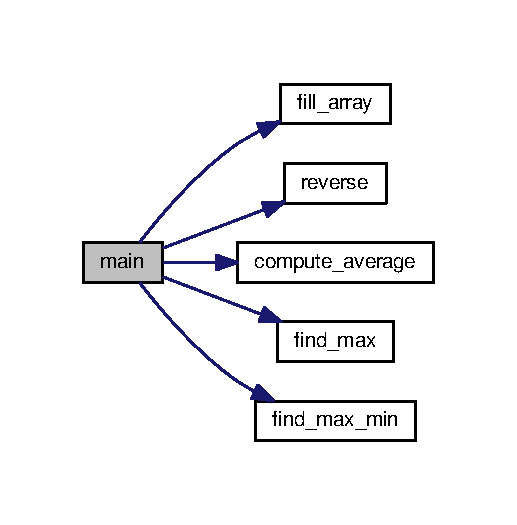
\includegraphics[width=248pt]{ArrayPractice_8cpp_ae66f6b31b5ad750f1fe042a706a4e3d4_cgraph}
\end{center}
\end{figure}


\index{Array\+Practice.\+cpp@{Array\+Practice.\+cpp}!reverse@{reverse}}
\index{reverse@{reverse}!Array\+Practice.\+cpp@{Array\+Practice.\+cpp}}
\subsubsection[{\texorpdfstring{reverse(const char a[], int num\+\_\+used)}{reverse(const char a[], int num_used)}}]{\setlength{\rightskip}{0pt plus 5cm}void reverse (
\begin{DoxyParamCaption}
\item[{const char}]{a\mbox{[}$\,$\mbox{]}, }
\item[{int}]{num\+\_\+used}
\end{DoxyParamCaption}
)}\hypertarget{ArrayPractice_8cpp_ad637601aeb87032b931bc689000f503a}{}\label{ArrayPractice_8cpp_ad637601aeb87032b931bc689000f503a}

\begin{DoxyCode}
56 \{
57    \textcolor{keywordflow}{for} (\textcolor{keywordtype}{int} k = num\_used - 1; k >= 0; k--)
58    \{
59       cout << a[k] << \textcolor{stringliteral}{", "};
60    \}
61    cout << endl;
62 \}
\end{DoxyCode}

%--- End generated contents ---

% Index
\backmatter
\newpage
\phantomsection
\clearemptydoublepage
\addcontentsline{toc}{chapter}{Index}
\printindex

\end{document}
